
\documentclass[a4,10pt]{ctexart}

\usepackage{ctex}
\usepackage[utf8]{inputenc}
\usepackage{amsfonts,amsmath,amscd,amssymb,amsthm}
\usepackage{latexsym,bm}
\usepackage{cite}
\usepackage{mathtools,mathdots,graphicx,array}
\usepackage{fancyhdr}
\usepackage{lastpage}
\usepackage{color}
\usepackage{enumitem}
\usepackage{mpdoc}
\usepackage{diagbox}
\usepackage{xcolor,tcolorbox,tikz,tkz-tab,mdframed,tikz-cd}
\usepackage{framed}
\usepackage{verbatim}
\usepackage{extarrows}
\usepackage{fontspec}
\newcommand*{\dif}{\mathop{}\!\mathrm{d}}
\newcommand*{\arsinh}{\mathop{}\!\mathrm{arsinh}}
\newcommand*{\artanh}{\mathop{}\!\mathrm{artanh}}
\newcommand*{\arcosh}{\mathop{}\!\mathrm{arcosh}}
\newcommand*{\Li}{\mathop{}\!\textrm{Li}}
\usepackage{minted}
\usepackage{fontspec}
\usepackage{amsmath}
\usepackage{fancyvrb} % for inline code
\usepackage{listings}

\usemintedstyle{xcode}

\begin{document}
\pagenumbering{roman}
\title{Notes}
\author{X.W.}
\date{2023年9月}
\maketitle
\tableofcontents
\newpage
\pagenumbering{arabic}
\newpage


\section{要做的事情}

\begin{yd}{积极锻炼身体日志}{}
	\begin{itemize}[noitemsep]
		\item 2023/9/4, 晚上跑步, 总计时间: 散步+跑步=52分钟
		\item 2023/9/5, 休息
		\item 2023/9/6, 休息
		\item 2023/9/7, 休息
		\item 2023/9/8, 休息
		\item 2023/9/9, 晚上跑步,总计时间:散步+跑步=50分钟
	\end{itemize}
\end{yd}

\begin{yd}{积极出去玩}{}
	\begin{itemize}[noitemsep]
		\item 2023/9/2--2023/9/4, 安徽省:潜山县:天柱山.
	\end{itemize}
\end{yd}

\begin{yd}{积极学习速写}{}
	\begin{itemize}[noitemsep]
		\item 希望有时间学学
	\end{itemize}
\end{yd}

\begin{yd}{积极阅读}{}
	\begin{itemize}[noitemsep]
		\item 心流: 最优体验, 待阅读(2023/9/4--)
	\end{itemize}
\end{yd}


\begin{yd}{阅读 \textbf{SICP}}{}
	\begin{itemize}[noitemsep]
		\item page 69: 层次性数据和闭包性质. 2023/9/4
	\end{itemize}
\end{yd}

\begin{yd}{阅读 \textbf{数据密集型应用系统设计}}{}
	\begin{itemize}[noitemsep]
		\item page 71: 数据存储与检索. 2023/9/4
	\end{itemize}
\end{yd}

\begin{yd}{阅读 \textbf{计算机网络}}{}
	\begin{itemize}[noitemsep]
		\item page 1: 计算机网络和因特网. 2023/9/4
	\end{itemize}
\end{yd}

\begin{yd}{阅读 \textbf{深入理解计算机系统}}{}
	\begin{itemize}[noitemsep]
		\item page 23: 信息的表示和处理. 2023/9/4
	\end{itemize}
\end{yd}

\begin{yd}{吹 \textbf{Nginx 和 Kong}}{}
	\begin{itemize}[noitemsep]
		\item 基本复现 Kong Demo. 2023/9/4
		\item 开始阅读 Nginx. 2023/9/7
	\end{itemize}
\end{yd}

\begin{yd}{吹 \textbf{SSO 登录}}{}
	\begin{itemize}[noitemsep]
		\item 看 IAM 代码. 2023/9/4
	\end{itemize}
\end{yd}

\begin{yd}{学习 \textbf{SpringBoot}}{}
	\begin{itemize}[noitemsep]
		\item 看代码. 2023/9/4
	\end{itemize}
\end{yd}

\begin{yd}{吹 \textbf{OpenTelemetry}}{}
	\begin{itemize}[noitemsep]
		\item 基本复现 NodeJS 中的使用. 2023/9/4
		\item 待看: \href{https://www.bilibili.com/video/BV1cN411a72d/?vd_source=3d6137a386838c2bcb88b1db7c993448}{K8S OpenTelemetry 分享} (2023/9/4--)
	\end{itemize}
\end{yd}

\section{Spring Note}

\section{Nginx Note}

\subsection{OpenResty Note}

OpenResty 是基于Nginx 和 LuaJIT 的Web开发平台。以下是其重点:

\begin{zy}
	\begin{itemize}[noitemsep]
		\item 同步非阻塞的编程模式;
		\item 不同阶段的作用;
		\item LuaJIT 和 Lua 的不同之处;
		\item OpenResty API 和周边库;
		\item 协程和 cosocket;
		\item 单元测试框架和性能测试工具;
		\item 火焰图和周边工具链;
		\item 性能优化。
	\end{itemize}
\end{zy}


\subsubsection{Nginx 概念}

如图 \ref{key4} 所示,Nginx启动之后,会有一个 Master 进程和多个 Worker 进程(也可以只有一个 Worker 进程,
取决于配置)。Master 进程不负责处理终端的请求。它是用来管理 Worker 进程的,
包括接受管理员发送的信号量、监控 Worker 的运行状态。当 Worker 进程异常退出时,
Master 进程会重新启动一个新的 Worker 进程。
Worker 进程用来处理终端用户的请求。它是从 Master 进程 fork 出来的,彼此之间相互独立,
互不影响,没有线程间加锁,也方便调试。即使某个进程崩溃退出了,也不会影响其他 Worker 进程正常工作。

\begin{figure}[htbp]
	\centering
	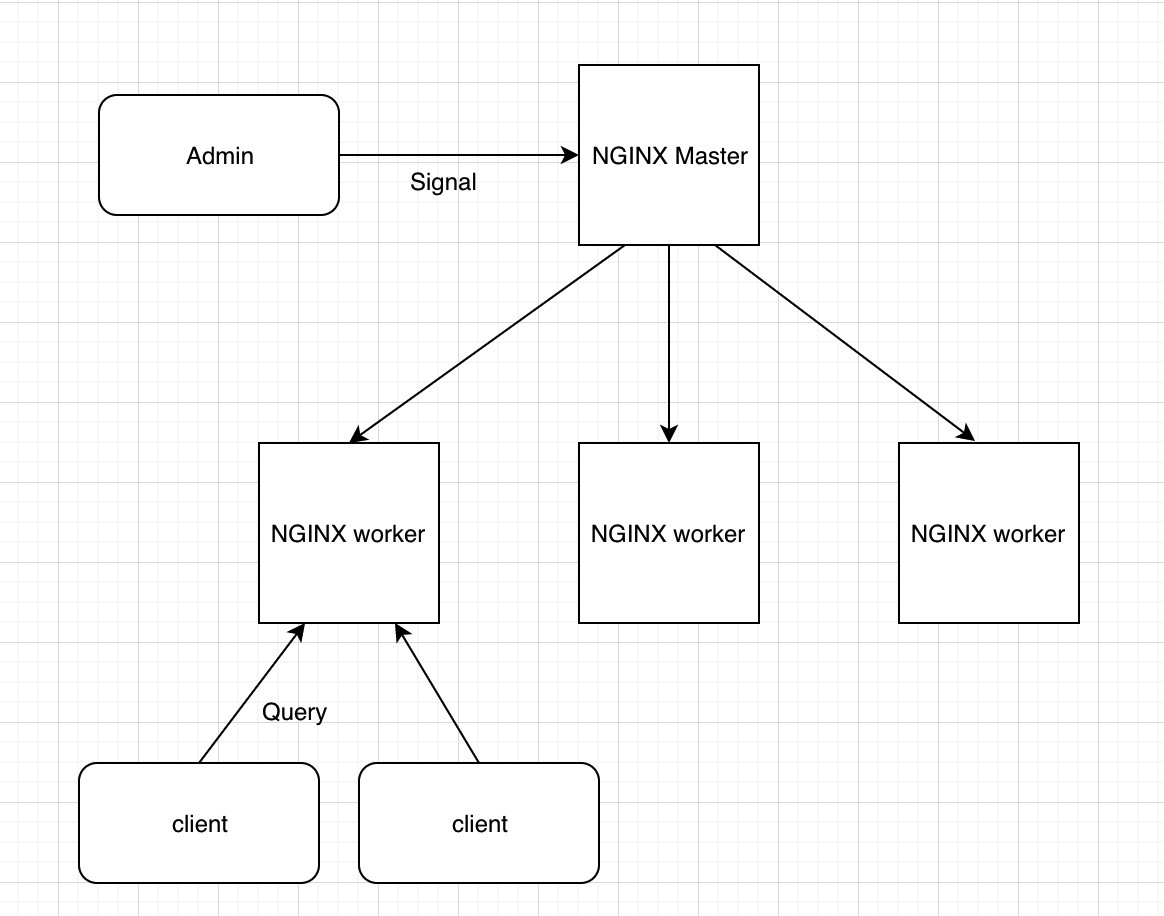
\includegraphics[width=.4\textwidth]{img/nginx/nginx_process.jpg}
	\caption{Nginx 多线程模式}
	\label{key4}
\end{figure}


OpenResty 在 Nginx Master-Worker 模式的前提下,
增加了独有的特权进程(privileged agent)。
这个进程并不监听任何端口,和 Nginx 的 Master 进程拥有同样的权限,
所以可以做一些需要高权限才能完成的任务,比如对本地磁盘文件的一些写操作等。

Nginx 一个典型的配置如下,每个指令都有自己的 context (上下文),
最上层的是 main,里面是和具体业务无关的一些指令,
比如上面出现的 worker\_processes、pid 和 error\_log,
都属于 main 这个上下文。另外,上下文是有层级关系的,
比如 location 的上下文是 server,server 的上下文是 http,http 的上下文是 main。
Nginx不仅可以处理 HTTP 请求 和 HTTPS 流量,还可以处理 UDP 和 TCP 流量。
其中,七层的放在 HTTP 中,四层的放在 stream中。
\begin{minted}[frame=lines,tabsize=4]{c++}
	worker_processes auto;
	pid logs/nginx.pid;
	error_log logs/error.log notice;
	worker_rlimit_nofile 65535;
	events {
		worker_connections 16384;
	}
	http {
		server {
			listen 80;
			listen 443 ssl;
			location / {
				proxy_pass https://foo.com;
			}
		}
	}
	stream {
		server {
			listen 53 udp;
		}
	}
\end{minted}

\subsubsection{OpenResty 概念}

结构如图 \ref{key5} 所示,其中 init\_by\_lua 只会在 Master 进程被创建时执行,
init\_worker\_by\_lua 只会在每个 Worker 进程被创建时执行。
其他的 *\_by\_lua 指令则是由终端请求触发,会被反复执行。

所以在 init\_by\_lua 阶段,可以预先加载 Lua 模块和公共的只读数据,
这样可以利用操作系统的 COW(copy on write)特性,来节省一些内存。

\begin{figure}[htbp]
	\centering
	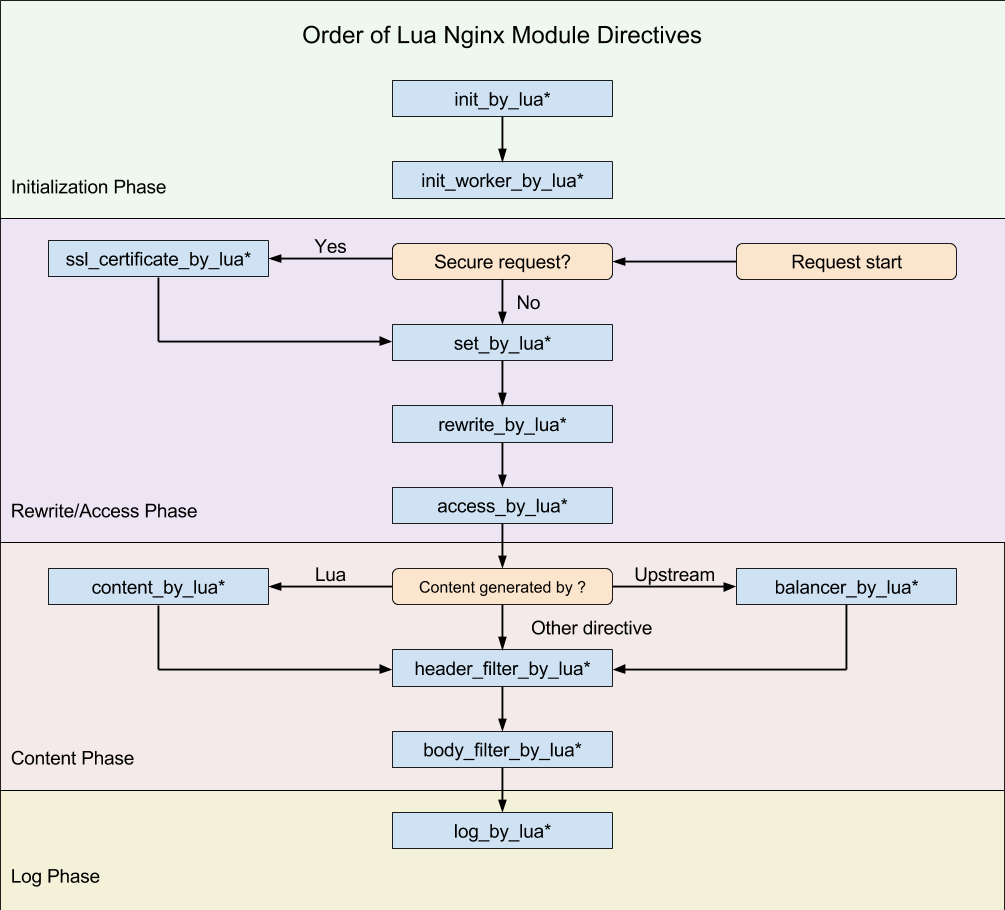
\includegraphics[width=.6\textwidth]{img/nginx/nginx_module.png}
	\caption{OpenResty Module}
	\label{key5}
\end{figure}

对于业务代码来说,其实大部分的操作都可以在 content\_by\_lua 里面完成,
更推荐的做法,是根据不同的功能来进行拆分,如下面所示,各个阶段的作用:
\begin{zy}
	\begin{itemize}[noitemsep]
		\item \textbf{set\_by\_lua}:设置变量;
		\item \textbf{rewrite\_by\_lua}:转发、重定向等;
		\item \textbf{access\_by\_lua}:准入、权限等;
		\item \textbf{content\_by\_lua}:生成返回内容;
		\item \textbf{header\_filter\_by\_lua}:应答头过滤处理;
		\item \textbf{body\_filter\_by\_lua}:应答体过滤处理;
		\item \textbf{log\_by\_lua}:日志记录。
	\end{itemize}
\end{zy}

\paragraph{LuaJIT 概念}

OpenResty 的 worker 进程都是 fork master 进程而得到的,
master 进程中的 LuaJIT 虚拟机也会一起 fork 过来。
在同一个 worker 内的所有协程,都会共享这个 LuaJIT 虚拟机,
Lua 代码的执行也是在这个虚拟机中完成的。

LuaJIT和Lua 的关系,标准 Lua 出于性能考虑,并不是直接被解释执行的,
而是先由 Lua 编译器编译为字节码(Byte Code),然后再由 Lua 虚拟机执行。
而 LuaJIT 的运行时环境,除了一个汇编实现的 Lua 解释器外,
还有一个可以直接生成机器代码的 JIT 编译器。
开始的时候,LuaJIT和标准 Lua 一样,Lua 代码被编译为字节码,
字节码被 LuaJIT 的解释器解释执行。不同的是,
\textbf{LuaJIT的解释器会在执行字节码的同时,记录一些运行时的统计信息,
比如每个 Lua 函数调用入口的实际运行次数,还有每个 Lua 循环的实际执行次数。
当这些次数超过某个随机的阈值时,便认为对应的 Lua 函数入口或者对应的 Lua 循环足够热,
这时便会触发 JIT 编译器开始工作。}

JIT 编译器会从热函数的入口或者热循环的某个位置开始,
尝试编译对应的 Lua 代码路径。编译的过程,
是把 LuaJIT 字节码先转换成LuaJIT 自己定义的中间码(IR),
然后再生成针对目标体系结构的机器码。LuaJIT 的性能优化,
本质上就是让尽可能多的 Lua 代码可以被 JIT 编译器生成机器码,
而不是回退到 Lua 解释器的解释执行模式。

LuaJIT 除了兼容 Lua 5.1 的语法并支持 JIT 外,
LuaJIT 还紧密结合了 FFI(Foreign Function Interface),
可以直接在 Lua 代码中调用外部的 C 函数和使用 C 的数据结构。

\begin{minted}[frame=lines,tabsize=4]{c++}
	local ffi = require("ffi")
	ffi.cdef[[
	int printf(const char *fmt, ...);
	]]
	ffi.C.printf("Hello %s!", "world")
\end{minted}

可以直接在 Lua 中调用 C 的 printf 函数,打印出 Hello world!。
可以用 FFI 来调用 Nginx、OpenSSL 的 C 函数,来完成更多的功能。
实际上,FFI 方式比传统的 Lua/C API 方式的性能更优。出于性能方面的考虑,
LuaJIT 还扩展了 table 的相关函数:table.new 和 table.clear。

在 Lua 中,可以使用 Lua C API 来调用 C 函数,而在 LuaJIT 中还可以使用 FFI。
对 OpenResty 而言:在核心的 lua-nginx-module 中,
调用 C 函数的 API,都是使用 Lua C API 来完成的;
而在 lua-resty-core 中,则是把 lua-nginx-module 已有的部分 API,
使用 FFI 的模式重新实现了一遍。

\subparagraph{Lua C function}

用 C 编写的函数,无法把返回值传给 Lua 代码,而是需要通过栈,
来传递 Lua 和 C 之间的调用参数和返回值。同时,这些代码也不能被 JIT 跟踪到,
所以对于 LuaJIT 而言,这些操作是处于黑盒中的,没法进行优化。
\begin{minted}[frame=lines,tabsize=4]{c++}
	static int ngx_http_lua_ngx_decode_base64(lua_State *L){
		ngx_str_t p, src;
		src.data = (u_char *) luaL_checklstring(L, 1, &src.len);
		p.len = ngx_base64_decoded_length(src.len);
		p.data = lua_newuserdata(L, p.len);
		if (ngx_decode_base64(&p, &src) == NGX_OK) {
			lua_pushlstring(L, (char *) p.data, p.len);
		} else {
			lua_pushnil(L);
		}
		return 1;
	}
\end{minted}

主要的是 ngx\_base64\_decoded\_length 和 ngx\_decode\_base64,
它们都是 Nginx 自身提供的 C 函数。对于那些能够被 Lua 调用的 C 函数来说,
它的接口必须遵循 Lua 要求的形式,
也就是 typedef int (*lua\_CFunction)(lua\_State* L)。
它包含的参数是 lua\_State 类型的指针 L;
它的返回值类型是一个整型,表示返回值的数量,而非返回值自身。

\begin{minted}[frame=lines,tabsize=4]{c++}
	static int ngx_http_lua_ngx_decode_base64(lua_State *L);
\end{minted}

\subparagraph{LuaJIT FFI}

FFI 的交互部分是用 Lua 实现的,这部分代码可以被 JIT 跟踪到,并进行优化。
LuaJIT 只负责由自己分配的资源;而 ffi.C 是 C 库的命名空间,
所以,使用 ffi.C 分配的空间不由 LuaJIT 负责,需要自己手动释放。

\begin{minted}[frame=lines,tabsize=4]{c++}
	ngx.decode_base64 = function (s)
		local slen = #s
		local dlen = base64_decoded_length(slen)
		local dst = get_string_buf(dlen)
		local pdlen = get_size_ptr()
		local ok = C.ngx_http_lua_ffi_decode_base64(s, slen, dst, pdlen)
	if ok == 0 then
		return nil
	end
		return ffi_string(dst, pdlen[0])
	end
\end{minted}

\paragraph{Lua 元表}

元表的表现行为类似于操作符重载,比如可以重载 \_\_add,来计算两个 Lua 数组的并集;
或者重载 \_\_tostring,来定义转换为字符串的函数。
Lua 提供了两个处理元表的函数,setmetatable(table, metatable), 
用于为一个 table 设置元表,getmetatable(table),用于获取 table 的元表。


\begin{minted}[tabsize=4,frame=lines]{c++}
	local _M = { _VERSION = '0.21' } -- 使用 table 模拟类
	local mt = { __index = _M } -- mt 即 metatable 的缩写,__index 指向类自身
	-- 类的构造函数
	function _M.new(self) 
		local sock, err = tcp()
		if not sock then
			return nil, err
		end
		return setmetatable({ sock = sock }, mt) -- 使用 table 和 metatable 模拟类的实例
	end
	-- 类的成员函数
	function _M.set_timeout(self, timeout) -- 使用 self 参数,获取要操作的类的实例
		local sock = self.sock
		if not sock then
			return nil, "not initialized"
		end
		return sock:settimeout(timeout)
	end
\end{minted}

\_M 这个 table 模拟了一个类,初始化时,它只有 \_VERSION 这一个成员变量,
并在随后定义了 \_M.set\_timeout 等成员函数。
在 \_M.new(self) 这个构造函数中,
返回了一个 table,这个 table 的元表就是 mt,而 mt 的 \_\_index 元方法指向了 \_M,
这样,返回的这个 table 就模拟了类 \_M 的实例。

\begin{minted}[tabsize=4,frame=lines]{c++}
	$ resty -e 'local tb = {}
	tb[1] = {red}
	tb[2] = function() print("func") end
	setmetatable(tb, {__mode = "v"})
	print(#tb)  -- 2
	collectgarbage()
	print(#tb) -- 0
	'
\end{minted}

当一个 table 的元表中存在 \_\_mode 字段时,这个 table 就是弱表(weak table)了。
如果 \_\_mode 的值是 k,那就意味着这个 table 的 键 是弱引用,\_\_mode 的值是 v,
那就意味着这个 table 的 值是弱引用。也可以设置为 kv,表明这个表的键和值都是弱引用。
这三者中的任意一种弱表,只要它的 \textbf{键} 或者 \textbf{值} 被回收了,
那么对应的整个键值 对象都会被回收。

\subsubsection{OpenResty 原理}

OpenResty 的 master 和 worker 进程中,都包含一个 LuaJIT VM。
在同一个进程内的所有协程,都会共享这个 VM,并在这个 VM 中运行 Lua 代码。
而在同一个时间点上,每个 worker 进程只能处理一个用户的请求,也就是只有一个协程在运行。
Nginx 能够支持 C10K (上万并发),实际上是通过 epoll 的事件驱动,
来减少等待和空转,才尽可能地让 CPU 资源都用于处理用户的请求。
毕竟,只有单个的请求被足够快地处理完,整体才能达到高性能的目的。
如果采用的是多线程模式,让一个请求对应一个线程,那么在 C10K 的情况下,资源很容易就会被耗尽的。

在 OpenResty 层面,Lua 的协程会与 Nginx 的事件机制相互配合。
如图 \ref{key6} 所示,如果 Lua 代码中出现类似查询 MySQL 数据库这样的 I/O 操作,
就会先调用 Lua 协程的 yield 把自己挂起,然后在 Nginx 中注册回调;
在 I/O 操作完成(也可能是超时或者出错)后,再由 Nginx 回调 resume 来唤醒 Lua 协程。
这样就完成了 Lua 协程和 Nginx 事件驱动的配合,避免在 Lua 代码中写回调。

\begin{figure}[htbp]
	\centering
	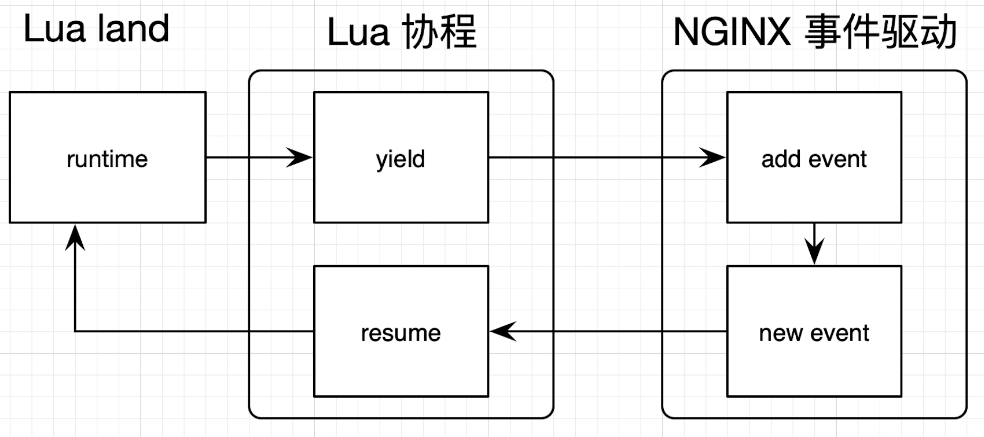
\includegraphics[width=.5\textwidth]{img/nginx/luaJIT_process.png}
	\caption{LuaJIT 与 Nginx 的相互配合}
	\label{key6}
\end{figure}

如果 Lua 代码中没有 I/O 或者 sleep 操作,比如全是密集的加解密运算,
那么 Lua 协程就会一直占用 LuaJIT VM,直到处理完整个请求。
例如 sleep 函数的具体实现。
需要先通过 C 函数 ngx\_http\_lua\_ngx\_sleep,来注册 ngx.sleep 这个 Lua API:

\begin{minted}[tabsize=4,frame=lines]{c++}
	void ngx_http_lua_inject_sleep_api(lua_State *L)
	{
		lua_pushcfunction(L, ngx_http_lua_ngx_sleep);
		lua_setfield(L, -2, "sleep");
	}
\end{minted}

sleep 的主函数主要的代码:

\begin{minted}[tabsize=4,frame=lines]{c++}
	static int ngx_http_lua_ngx_sleep(lua_State *L){
		coctx->sleep.handler = ngx_http_lua_sleep_handler;
		ngx_add_timer(&coctx->sleep, (ngx_msec_t) delay);
		return lua_yield(L, 0);
	}
\end{minted}

可以看到这里先增加了 ngx\_http\_lua\_sleep\_handler 这个回调函数;
然后调用 ngx\_add\_timer 这个 Nginx 提供的接口,向 Nginx 的事件循环中增加一个定时器;
最后使用 lua\_yield 把 Lua 协程挂起,把控制权交给 Nginx 的事件循环。
当 sleep 操作完成后, ngx\_http\_lua\_sleep\_handler 这个回调函数就被触发了。
它里面调用了 ngx\_http\_lua\_sleep\_resume, 并最终使用 lua\_resume 唤醒了 Lua 协程。

\paragraph{OpenResty cosocket}

cosocket是 OpenResty 中的专有名词,是把协程和网络套接字的英文拼在一起形成的,
即 cosocket = coroutine + socket。所以,可以把 cosocket 翻译为“协程套接字”。
cosocket 不仅需要 Lua 协程特性的支持,
也需要 Nginx 中非常重要的事件机制的支持,这两者结合在一起,
最终实现了非阻塞网络 I/O。另外,cosocket 支持 TCP、UDP 和 Unix Domain Socket。

OpenResty 以此图 \ref{key6},封装实现 connect、send、receive 等操作,
形成了 cosocket API以处理 TCP 的 API 为例来处理 UDP 和 Unix Domain Socket ,
与TCP 的接口基本是一样的。相关的TCP的API接口如下:

\begin{itemize}[noitemsep]
	\item 创建对象:ngx.socket.tcp。
	\item 设置超时:tcpsock:settimeout 和 tcpsock:settimeouts。
	\item 建立连接:tcpsock:connect。
	\item 发送数据:tcpsock:send。
	\item 接受数据:tcpsock:receive、tcpsock:receiveany 和 tcpsock:receiveuntil。
	\item 连接池:tcpsock:setkeepalive。
	\item 关闭连接:tcpsock:close。
\end{itemize}

如下列的代码,通过 ngx.socket.tcp(),创建 TCP 的 cosocket 对象,使用 settimeout() ,
把超时时间设置为 1 秒。注意这里的超时没有区分 connect、receive,是统一的设置。
使用 connect() 去连接指定网站的 80 端口,如果失败就直接退出。
连接成功的话,就使用 send() 来发送构造好的数据,如果发送失败就退出。
发送数据成功的话,就使用 receive() 来接收网站返回的数据。
这里 receive() 的默认参数值是 *l,也就是只返回第一行的数据;
如果参数设置为了*a,就是持续接收数据,直到连接关闭;
最后,调用 close() ,主动关闭 socket 连接。

\begin{minted}[tabsize=4,frame=lines]{c++}
	$ resty -e 'local sock = ngx.socket.tcp()
        sock:settimeout(1000)  -- one second timeout
        local ok, err = sock:connect("www.baidu.com", 80)
        if not ok then
            ngx.say("failed to connect: ", err)
            return
        end

        local req_data = "GET / HTTP/1.1\r\nHost: www.baidu.com\r\n\r\n"
        local bytes, err = sock:send(req_data)
        if err then
            ngx.say("failed to send: ", err)
            return
        end

        local data, err, partial = sock:receive()
        if err then
            ngx.say("failed to receive: ", err)
            return
        end

        sock:close()
        ngx.say("response is: ", data)'
\end{minted}





OpenResty 的实现中,只有 shared dict 可以完成 worker 间的数据共享,
并借此实现 worker 之间的通信,这也是它存在的价值。对外提供了 20多个 Lua API,
所有的这些 API 都是原子操作。








\section{JS Note}

\section{MySQL Note}

\subsection{MySQL 概述}

\begin{figure}[htbp]
	\centering
	
\includegraphics[width=.6\textwidth]{img/mysql/1/dbConnect.png}
	\caption{MySQL与系统的交互}
	\label{key1}
\end{figure}

如图 \ref{key1} 所示,访问数据库需要和数据库建立一个网络连接,
MySQL驱动会在底层跟数据库建立网络连接,接着发送请求给数据库服务器。

\begin{figure}[htbp]
	\centering
	\includegraphics[width=.6\textwidth]{img/mysql/1/executeSQL.png}
	\caption{SQL执行过程}
	\label{key2}
\end{figure}

网络链接由一个线程去进行处理,监听请求以及读取请求数据,
比如从网络连接中读取和解析出来一条系统发送过去的SQL语句。
如图 \ref{key2} 所示,当线程从网络连接中读取到SQL语句后,
转交给SQL Interface为执行SQL语句的接口,专门用于执行SQL语句。
查询解析器(Parser)就是负责对SQL语句进行解析的,所谓的SQL解析,就是按照既定的SQL语法,
按照SQL语法规则编写的SQL语句进行解析。
\textbf{通过解析器理解了SQL语句之后,接着会找查询优化器(Optimizer)来选择一个最优的查询路径。} 
把查询优化器选择的最优查询路径,也就是按照一个什么样的顺序和步骤去执行这个SQL语句的计划,
把这个计划交给底层的存储引擎去真正的执行。
\textbf{存储引擎其实就是执行SQL语句的,按照一定的步骤去查询内存缓存数据,更新磁盘数据,
查询磁盘数据,等等,执行诸如此类的一系列的操作。} 存储引擎支持各种各样的存储引擎的,
常见的InnoDB、MyISAM、Memory等等。MySQL一般是使用InnoDB存储引擎,执行器为根据执行计划调用存储引擎的接口。

\subsection{InnoDB 引擎}
\subsubsection{InnoDB 结构概述}

如图 \ref{key3} 所示,缓冲池会缓存很多数据,以便于以后的查询,当缓存池中存在的数据,就可以不用去查磁盘。

\begin{figure}[htbp]
	\centering
	
\includegraphics[width=.6\textwidth]{img/mysql/2/bufferPool.png}
	\caption{InnoDB 结构图}
	\label{key3}
\end{figure}

InnoDb 中的SQL执行流程, 可以通过以下SQL语句的执行表现出来:

\begin{minted}[frame=lines,tabsize=4]{cpp}
	update users set name="lihua" where id = 10;
\end{minted}







\section{杂记}

\section{常用环境}

\begin{zs}
        
这是一个注释
    
\end{zs}
    
\begin{xt}
        
这是一个习题.
    
\end{xt}
    
\begin{lt}
        
这是一个问题.
    
\end{lt}

\begin{yl}
        
这是一个引理.
    
\end{yl}

\begin{dl}{A}{}
        
这是一个定理.
    
\end{dl}
    
\begin{tl}{A}{}
        
这是一个推论.
    
\end{tl}

\begin{dy}{A}{}
        
这是一个定义.
    
\end{dy}

\begin{jl}{A}{}
        
这是一个结论.
    
\end{jl}

\begin{mt}{A}{}
        
这是一个命题.
    
\end{mt}

\begin{ti}{A}{}
        
这是一个题目.
    
\end{ti}

\begin{cx}{A}{}
        
这是一个猜想.
    
\end{cx}

\begin{zy}
        
这是注意.
    
\end{zy}

\begin{ts}
        
这是一点提示.
    
\end{ts}

\begin{lt}
        
这是一个例题.
    
\end{lt}

\begin{proof}
你还可以加一点证明. 
\end{proof}

我们注意到, 所有的数学公式将自动转换成行间公式的大小, 比如${1\over 2^k}$, $\sum_{i=0}^{998244353}i$. 

\section{起源与未来的修改计划}

起源与hkmod的模板, 添加了一些常用的标志词. 可以在mpdoc.sty里面进行更改, 相信根据注释你也会. 

使用愉快! 


\end{document}
